% !TEX root = ./informe.tex
\section{Búsqueda Local}

\subsection{Explicación}

Búsqueda local es una estrategia utilizada para mejorar una solución obtenida con una heurística. La idea general es dar una definición de vecindad para toda solución (por ejemplo, si mis soluciones son nodos, los vecinos pueden ser sus adyacentes), y buscar el candidato óptimo dentro de ese conjunto. Este proceso puede repetirse para tender hacia un máximo local. \\

Para este problema, consideramos como vecinos de un clique aquellos cliques que pueden obtenerse aplicando una operación de swap (reemplazar un nodo en el clique por uno que no está), una operación de agregado (de un nodo) o una operación de borrado (de un nodo). En cada iteración del algoritmo, reviso toda la vecindad y me quedo con el clique de mayor frontera.


\subsection{Pseudocódigo}

Las funciones EsClique() y Frontera() no son incluidas aquí por ser iguales a las incluidas previamente. Las complejidades son $O(n^3)$ y $O(n^2)$ respectivamente. \\

\begin{algorithm}[H]
\begin{algorithmic}
\Function{Resolver}{$solucion$, $iteraciones$}          \Comment $O(iteraciones * n^5)$

    \State $fronteraMaxima \gets$ Frontera($solucion$)                      \Comment $O(n^2)$
    \For{$i \in [1..iteraciones]$ }                                         \Comment $O(iteraciones * n^5)$
        \State $solucionActual \gets$ BusquedaLocal($solucion$)             \Comment $O(n^5)$
        \State $fronteraActual \gets$ Frontera($solucionActual$)            \Comment $O(n^2)$

        \If{$fronteraActual > fronteraMaxima$}                              \Comment $O(1)$
            \State $fronteraMaxima \gets fronteraActual$                    \Comment $O(1)$
            \State $solucion \gets solucionActual$                          \Comment $O(1)$
        \EndIf
    \EndFor
    \State return $solucion$

\EndFunction
\end{algorithmic}
\end{algorithm}

En nuestra búsqueda local, dado una solucion tratamos de movernos a la mejor solucion posible de la vecindad. Consideramos que nuestra vecindad de soluciones es aquella formada por las que tienen un nodo swapeado, un nodo extra, o un nodo menos. La solución final de la búsqueda local es la mejor de las tres posibilidades de nuestra vecindad. \\

\begin{algorithm}[H]
\begin{algorithmic}
\Function{BusquedaLocal}{$solucionInicial$}             \Comment $O(n^5)$
    \State $complementoInicial \gets$ Complemento($solucionInicial$) \Comment $O(n)$\\

    \State $solucionSwap \gets$ MaximoPorSwap($solucionInicial$, $complementoInicial$)  \Comment $O(n^5)$
    \State $fronteraSwap \gets$ Frontera($solucionSwap$)                                \Comment $O(n^2)$ \\

    \State $solucionAdd \gets$ MaximoPorAdd($solucionInicial$, $complementoInicial$)    \Comment $O(n^4)$
    \State $fronteraAdd \gets$ Frontera($solucionAdd$)                                  \Comment $O(n^2)$\\

    \State $solucionSub \gets$ MaximoPorSub($solucionInicial$)      \Comment $O(n^4)$
    \State $fronteraSub \gets$ Frontera($solucionSub$)              \Comment $O(n^2)$\\

    \State $solucionSuprema \gets solucionSwap$ \Comment $O(1)$
    \State $fronteraSuprema \gets fronteraSwap$ \Comment $O(1)$\\

    \If{$fronteraAdd > fronteraSuprema$}                \Comment $O(1)$
        \State $fronteraSuprema \gets$ $fronteraAdd$    \Comment $O(1)$
        \State $solucionSuprema \gets$ $solucionAdd$    \Comment $O(1)$\\
    \EndIf

    \If{$fronteraSub > fronteraSuprema$}                \Comment $O(1)$
        \State $fronteraSuprema \gets$ $fronteraSub$    \Comment $O(1)$
        \State $solucionSuprema \gets$ $solucionSub$    \Comment $O(1)$\\
    \EndIf

    \State return $solucionSuprema$                     \Comment $O(1)$
\EndFunction

\end{algorithmic}
\end{algorithm}

Al swappear no nos quedamos con el primer swappeo que se pueda, sino que vemos las $n^2$ combinaciones de swaps para elegir la mejor (siempre que el swap mantenga una clique solución).

\begin{algorithm}[H]
\begin{algorithmic}
\Function{MaximoPorSwap}{$solucionInicial$, $complementoInicial$}   \Comment $O(n^5)$

    \State $candidatos \gets solucionInicial$
    \State $maxFrontera \gets$ Frontera($solucionInicial$)  \Comment $O(n^2)$
    \State $max\_i \gets -1$                                \Comment $O(1)$
    \State $max\_j \gets -1$                                \Comment $O(1)$\\

    \For{$i \in [0..|solucionInicial|)$}                    \Comment $O(n^5)$ Ver sección Complejidad
        \For{$j \in [0..|complementoInicial|)$}

            \State $candidato$[$i$] $\gets complementoInicial$[$j$] \Comment Hacemos swap $O(1)$

            \If{EsClique($candidatos$)}                                         \Comment $O(n^3)$
                \State $fronteraCandidato \gets$ Frontera($candidato$)          \Comment $O(n^2)$
                \If{$fronteraCandidato > maxFrontera$}                          \Comment $O(1)$
                    \State $max\_i \gets i$                                     \Comment $O(1)$
                    \State $max\_j \gets j$                                     \Comment $O(1)$
                    \State $maxFrontera \gets fronteraCandidato$                \Comment $O(1)$
                \EndIf
            \EndIf

            \State $candidato$[$i$] $\gets solucionInicial$[$j$] \Comment Restauro swap $O(1)$
        \EndFor
    \EndFor

    \If{$max\_i \neq -1$}                           \Comment $O(1)$
        \State $candidato$[$max\_i$] $\gets$ $complementoInicial$[$max\_j$] \Comment Swapeo definitivamente $O(1)$
    \EndIf

    \State return $candidatos$                      \Comment $O(1)$

\EndFunction
\end{algorithmic}
\end{algorithm}

En ``MaximoPorSub'' calculamos la frontera al sacar un único nodo (lo hacemos para todos los nodos) y vemos si la frontera aumenta. Puede pasar que al disminuir el tamaño de una clique queden muchas aristas ``libres'' que hagan que la frontera aumente. Probamos con todos y nos quedamos con la respuesta que mejoró la frontera, si es que hubo alguna.

\begin{algorithm}[H]
\begin{algorithmic}
\Function{MaximoPorSub}{$solucionInicial$}                      \Comment $O(n^4)$
    \State $candidatos \gets solucionInicial$
    \State $maxFrontera \gets$ Frontera($solucionInicial$)      \Comment $O(n^2)$
    \State $max\_c \gets -1$  \\                                \Comment $O(1)$

    \For{$c \in candidatos$}                                                \Comment $O(n^4)$
        \If{EsClique($candidatos - \{c\}$)}                                 \Comment $O(n^3)$
            \State $fronteraCandidato \gets$ Frontera($candidatos - \{c\}$) \Comment $O(n^2)$
            \If{$fronteraCandidato > maxFrontera$}                          \Comment $O(1)$
                \State $max\_c \gets c$                                     \Comment $O(1)$
                \State $maxFrontera \gets fronteraCandidato$                \Comment $O(1)$ \\
            \EndIf
        \EndIf
    \EndFor

    \If{$max\_c \neq -1$}                                           \Comment $O(1)$
        \State $candidatos \gets (candidatos - \{max\_c\})$         \Comment $O(1)$
    \EndIf

    \State return $candidatos$

\EndFunction
\end{algorithmic}
\end{algorithm}

En ``MaximoPorAdd'' probamos agregar de a un nodo, viendo que forme clique y calculando la nueva frontera. Si la frontera aumenta, nos guardamos la nueva solución.

\begin{algorithm}[H]
\begin{algorithmic}
\Function{MaximoPorAdd}{$solucionInicial$, $complementoInicial$}        \Comment $O(n^4)$

    \State $maxFrontera \gets$ Frontera($solucionInicial$)              \Comment $O(n^2)$
    \State $max\_c \gets -1$                                            \Comment $O(1)$
    \State $candidatos \gets solucionInicial$                           \Comment $O(1)$\\

    \For{$c \in complementoInicial$}                                            \Comment $O(n^4)$
        \If{EsClique($candidatos + \{c\}$)}                                     \Comment $O(n^3)$
            \State $fronteraCandidato \gets$ Frontera($candidatos + \{c\}$)     \Comment $O(n^2)$
            \If{$fronteraCandidato > maxFrontera$}                              \Comment $O(1)$
                \State $max\_c \gets c$                                         \Comment $O(1)$
                \State $maxFrontera \gets fronteraCandidato$                    \Comment $O(1)$\\
            \EndIf
        \EndIf
    \EndFor

    \If{$max\_c \neq -1$}                                           \Comment $O(1)$
        \State $candidatos \gets (candidatos + \{max\_c\})$         \Comment $O(1)$
    \EndIf

    \State return $candidatos$                      \Comment $O(1)$

\EndFunction
\end{algorithmic}
\end{algorithm}

Para calcular el complemento, armamos un vector de booleanos que dicen si un nodo pertenece o no a la solución input. Luego recorremos el vector y armamos un nuevo vector con aquellos nodos que no estaban en la solución original.

\begin{algorithm}[H]
\begin{algorithmic}
\Function{Complemento}{$solucionInicial$}
    \State $pertenece[i] =$ True $\iff i \in solucionInicial$   \Comment $O(n)$
    \State $complemento \gets \{\}$                             \Comment $O(1)$

    \For{$i \in [0..n)$}                                        \Comment $O(n)$
        \If{$pertenece$[$i$]$ = $True}                          \Comment $O(1)$
            \State $complemento$.PushBack($i$)                  \Comment $O(1)$  amortizado
        \EndIf
    \EndFor

    \State return $complemento$                                 \Comment $O(1)$

\EndFunction
\end{algorithmic}
\end{algorithm}


\subsection{Complejidad}

Las complejidades de cada linea fueron marcadas en el pseudocódigo, por lo que calcular la complejidad total es bastante sencillo.

\begin{itemize}
    \item MaximoPorAdd: $O(n^4)$. Son $O(n)$ iteraciones de algo $O(n^3)$.
    \item MaximoPorSub: $O(n^4)$. Son $O(n)$ iteraciones de algo $O(n^3)$.
    \item MaximoPorSwap: $O(n^5)$. El primer For recorre un vector $v$ y el For anidado recorre su complemento. Si consideramos que $|v| = \frac{n}{2}$, entonces el tamaño del complemento también es $\frac{n}{2}$, por lo que en total se recorren $O(n^2)$ elementos. Son $O(n^2)$ iteraciones de algo $O(n^3)$.
    \item BusquedaLocal: $O(n^5)$. Esto es por la complejidad de MaximoPorSwap que es la mayor, todo el resto es $O(n^4)$ o menor.
    \item Resolver: $O(\#iteraciones * n^5)$. Son $\#iteraciones$ veces de BusquedaLocal.
\end{itemize}

Por lo tanto, mejorar una solución inicial con este algoritmo de búsqueda local cuesta $O(\#iteraciones * n^5)$.

\subsection{Optimalidad}

Algo que notamos al probar este método es que el algoritmo goloso presentado en la sección anterior ya llega a un máximo local, por lo que es redundante aplicarle una búsqueda local para mejorarla. ¿Por qué ocurre esto? Porque si hubiera un nodo al que swappear con alguna de afuera para conseguir una mejor frontera, como este algoritmo siempre se queda con el mejor nodo fuera del clique, entonces el nodo de afuera ya tendría que estar dentro del clique. Tampoco podemos agregar nodos, pues si pudiesemos tomar más, el algoritmo goloso ya lo hubiera hecho. \todo{Mmm... No se me ocurre que pasa con Sub} \\

Sin embargo, aún así podemos encontrarle un uso. En la sección de Optimalidad del algoritmo goloso notamos que la diferencia entre la solución proporcionada por el algoritmo y la solución real puede ser arbitrariamente grande, con lo cuál pueden haber casos muy malos para nuestro algoritmo. Una forma de paliar este problema es que el algoritmo tome como entrada un nodo inicial, y que a partir de ahí construya una solución golosa. Llamaremos a esta variante $golosoB$, y al original $golosoA$. Por cuestiones de tiempo y del alcance de este informe no detallaremos la implementación de $golosoB$, pero es el algoritmo que motivará los apartados Búsqueda Local y Metaheurística. Sin embargo, no es más que lo que acabamos de decir, es sencillamente fijar un nodo incial antes de aplicar el algoritmo. \\

¿Por qué sirve nuestro algoritmo de búsqueda local para $golosoB$? Esto ocurre porque el primer nodo no fue elegido golosamente, es un nodo que fijamos en nuestra solución. Como consecuencia, una vez que la solución golosa queda construida, eliminar o swappear el primer nodo podría llegar producir un aumento en la frontera (agregar no, pues el algoritmo goloso siempre llega a un máximo local respecto a esta operación). Si esto llegase a ocurrir, aparecerían nuevos nodos candidatos a entrar en nuestra solución que no podiamos tomar antes porque no estaban conectados con el primer nodo. De esta forma, podemos continuar moviéndonos por las soluciones para llegar a algún máximo local mejor que el nos devolvió $golosoB$. \\

Tomemos el mismo ejemplo que complicaba a $golosoA$ utilizando $golosoB$ y \textit{búsquedaLocal}. \\

{\centering
    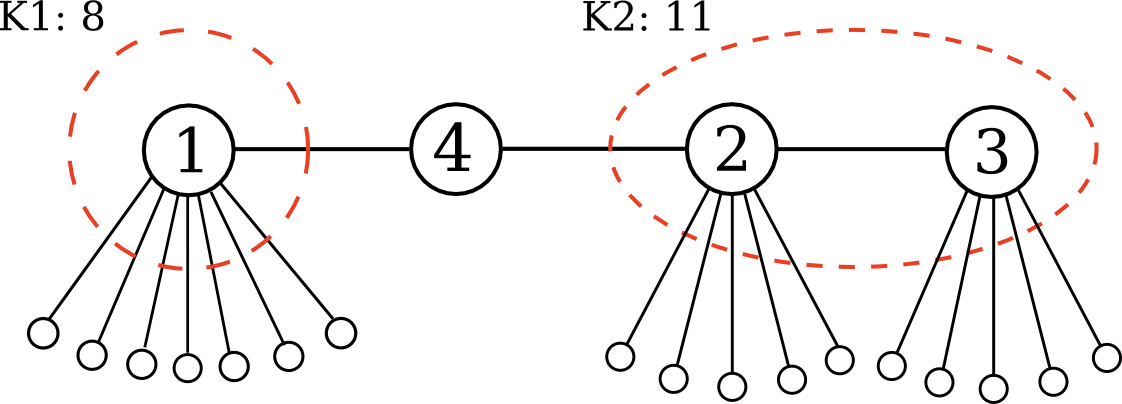
\includegraphics[width=0.57\textwidth]{informe/imgs/greedy_base_nodes_v2.png} \\
}
$ $\newline

Si a $golosoB$ le pasamos como entrada un nodo perteneciente al arbol $1$, o el nodo $4$; es imposible mejorar la solución de $golosoA$. Es el riesgo que tenemos al dejar libre el nodo inicial. \textit{Explicaremos este caso al final de la sección.} Sin embargo, si elegimos un nodo cualquiera del arbol $2$ o $3$, la situación es distinta. \\

El caso facil es si elegimos $2$ o $3$, en donde $golosoB$ se queda con la solución $(2,3)$, ya que ni las hojas ni el cuatro generan un clique con mayor frontera que ese par de nodos. \\

Más complicado es lo que ocurre al tomar una hoja de los arboles $2$ y $3$ como inicial. Asumamos que tomamos una hoja del $2$ (tomar una hoja del $3$ es análogo). La hoja sólo está conectada con el $2$, por lo que el $2$ se incluye en la solución. Una vez realizado esto, como nadie más está conectado con la hoja, \textit{golosoB} devuelve $(hoja,2)$. Es en este caso en donde \textit{búsquedaLocal} ayuda, pues a partir de $(hoja,2)$ busca los cliques que se pueden obtener haciendo swaps, con lo cual considera como candidato al clique producto de swappear la $hoja$ con el $2$, que es el clique $(2,3)$. Al ser la solución óptima, el algoritmo la toma en la primera iteración, y corta en la segunda. Termina devolviendo lo que queriamos: $(2,3)$. \\

{\centering
    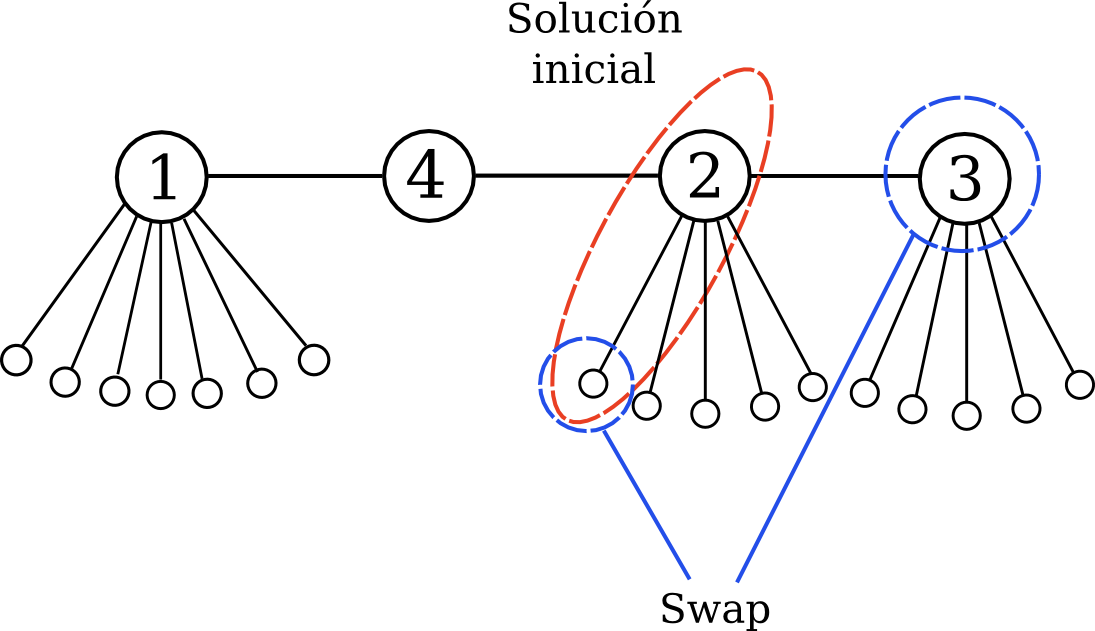
\includegraphics[width=0.57\textwidth]{informe/imgs/local_base_nodes_v2.png} \\
}
$ $\newline

{\centering
    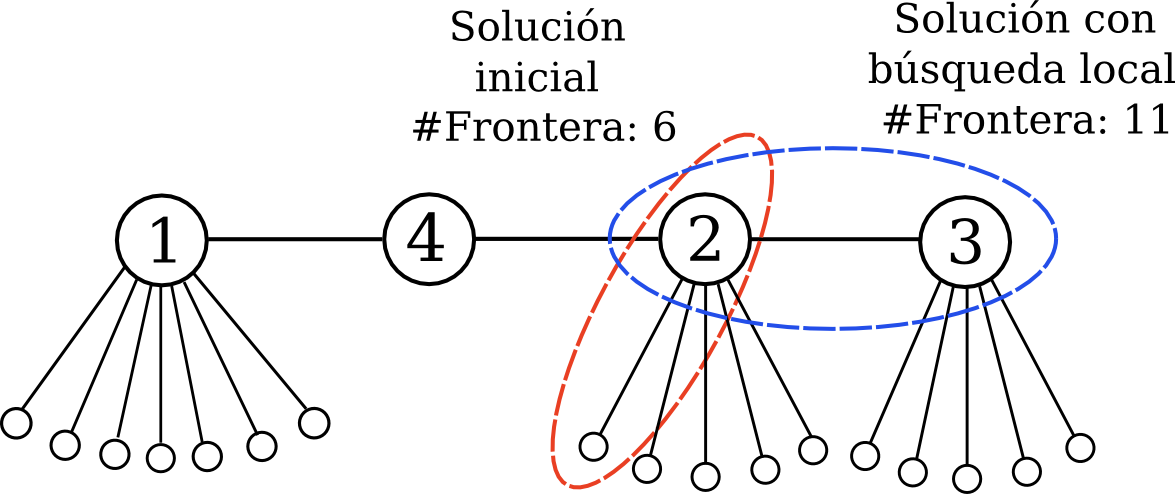
\includegraphics[width=0.57\textwidth]{informe/imgs/local_base_nodes_v3.png} \\
}
$ $\newline

Retomando lo mencionado hace unos párrafos, ¿que sucede si se elije un nodo del árbol $1$? Claramente $golosoB$ se vuelve tan malo como $golosoA$, pero \textbf{existe una solución muy sencilla}: podríamos elegir al azar el nodo inicial y correr el algoritmo muchas veces, para quedarnos con la mejor. Exploraremos esta idea en la última sección del informe: $GRASP$.

\subsection{Experimentación}
\todo[inline]{HABLAR DE LAS IMAGENES. inputs malos blabla}


{\centering
    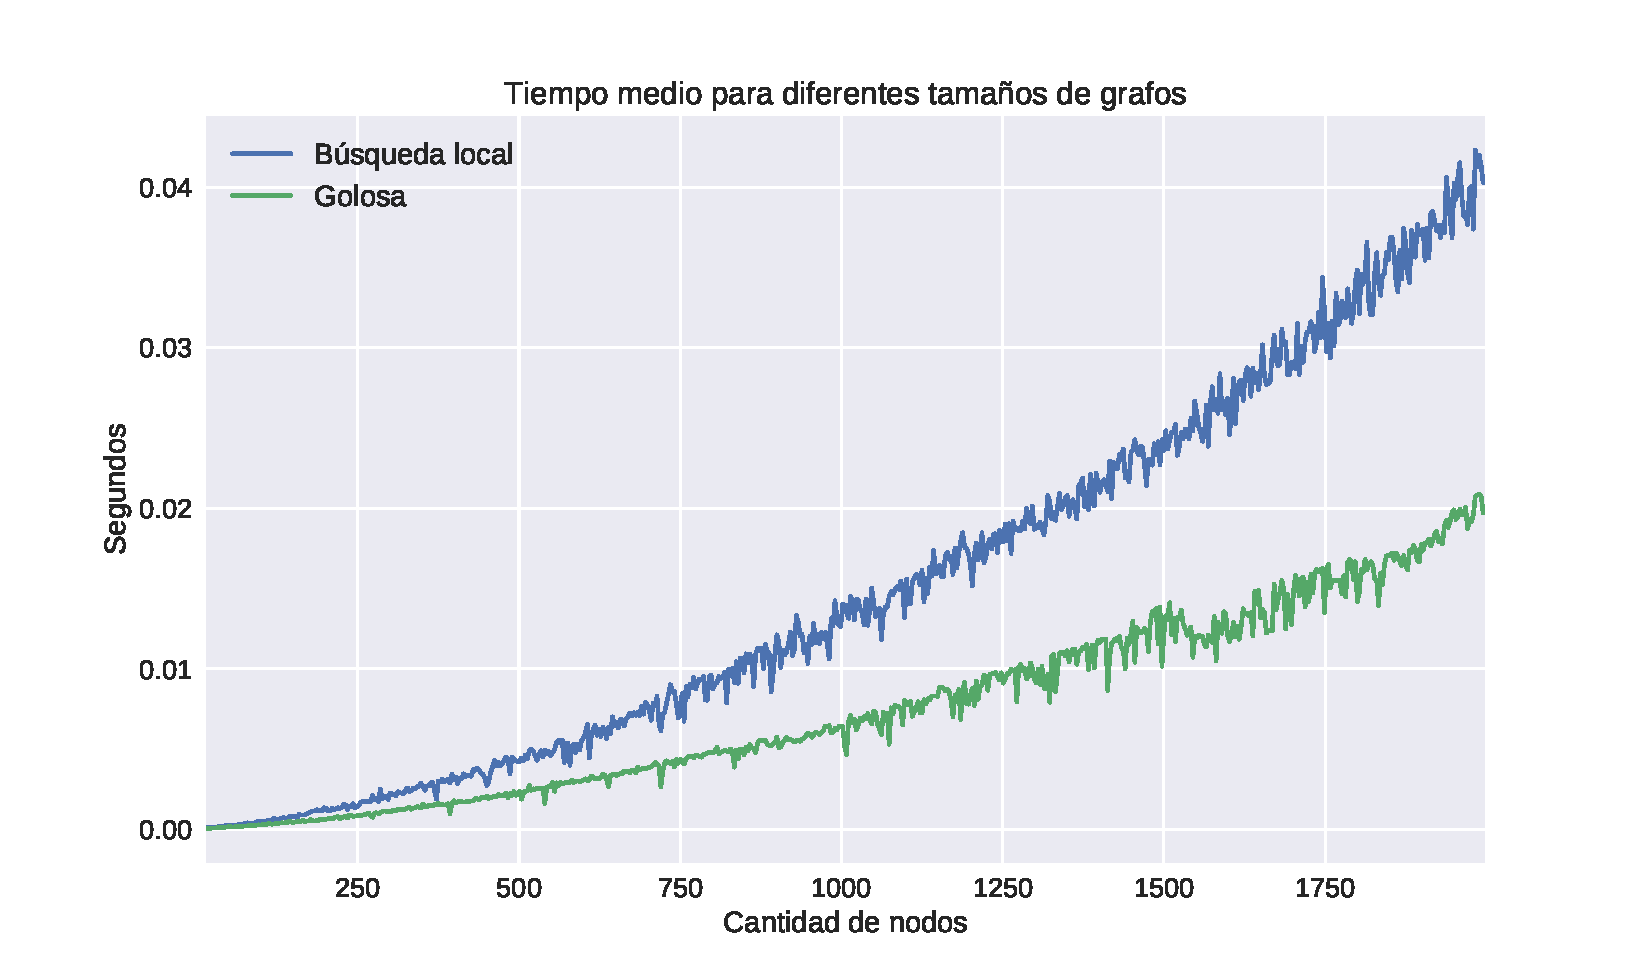
\includegraphics[width=1\textwidth]{informe/imgs/exp_malo_tiempo_greedy_local.pdf} \\
}
$ $\newline

{\centering
    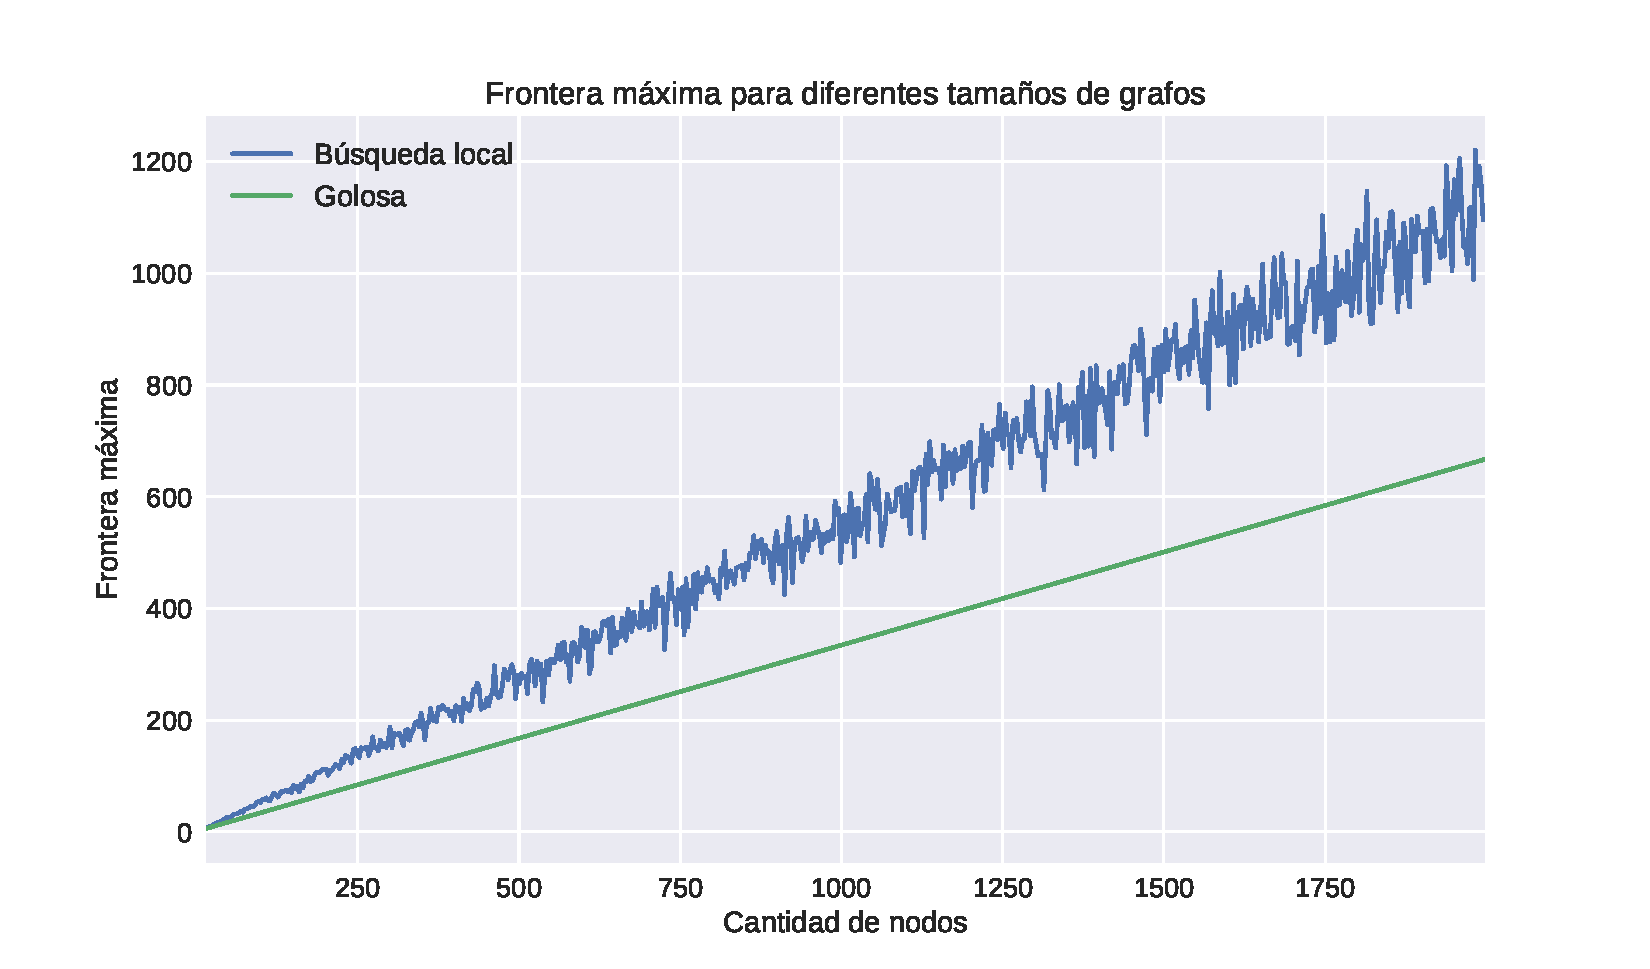
\includegraphics[width=1\textwidth]{informe/imgs/exp_malo_frontera_greedy_local.pdf} \\
}
$ $\newline